\section{Fusionswahrscheinlichkeiten}

\begin{frame}{Fusion als Energiequelle}
    \begin{columns}
        \begin{column}{0.55\textwidth}
            \begin{itemize}
                \item<+-> Unterschiedliche Fusionen für Wasserstoffisotope
                \item<+-> Produkte: $\gamma$-Strahlung und Helium
                \item<+-> Reaktion, wenn Coulomb-Abstoßung der Kerne überwunden wird
            \end{itemize}
        \end{column}
        \begin{column}{0.45\textwidth}
            \begin{center}
                \only<1->{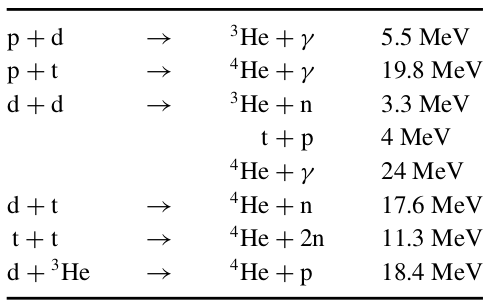
\includegraphics[width=0.75\textwidth]{images/Fusionsprozesse.png}
                \small{Interessante Fusionsprozesse mit schwerem Wasserstoff             \cite{Naga03}}}
            \end{center}
        \end{column}
    \end{columns}
    
    \only<3->{\textbf{Vorteile:}}
    \begin{itemize}
        \item<+-> Beinahe unbegrenzte Beschaffbarkeit der Rohstoffe (D, T) in Meer und Flüssen
        \item<+-> Quasi kein $\mathrm{CO_2}$-Ausstoß
        \item<+-> Kaum Produktion (langlebiger) radioaktiver Produkte
    \end{itemize}
    \only<6->{\textbf{Nachteile:}}
    \begin{itemize}
        \item<+-> Einen kontinuierlichen Fusionsprozess zu erzeugen und am Laufen zu halten ist nur schwer umsetzbar
    \end{itemize}
\end{frame}

\begin{frame}{Das Problem mit der Fusion}
    \begin{columns}
        \begin{column}{0.55\textwidth}
            \begin{itemize}
                \item<+-> Coulomb-Potential: \begin{align}V_C(r) = \frac{1}{4 \pi \varepsilon_0} \frac{q_1*q_2}{r}\end{align} Kernkräfte im Bereich $r < R_K \approx \SI{1}{\femto\m}$
                \item<+-> 2 Kerne können Barriere durch Tunneln überwinden
                \item<+-> Trotzdem erforderlich:
                \begin{itemize}
                    \item<+-> Erzeugung sehr hoher Temperaturen (Sonne)
                    \item<+-> Verwendung eines Katalysators
                \end{itemize}
            \end{itemize}
        \end{column}
        \begin{column}{0.45\textwidth}
            \begin{center}
                \only<1->{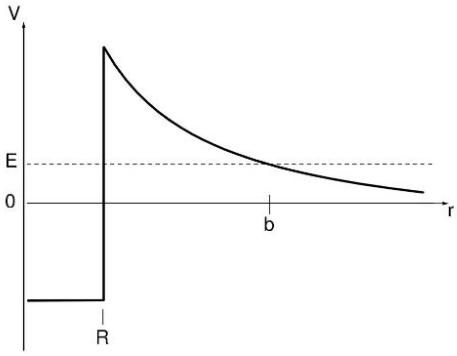
\includegraphics[width=\textwidth]{images/Potential.png}
                
                \small{Coulomb Potential \cite{IK4}}}
            \end{center}
        \end{column}
    \end{columns}
\end{frame}

\begin{frame}{Tunnelwahrscheinlichkeiten}
    \begin{itemize}
        \item<+-> Tunnelwahrscheinlichkeit mit $V(r) = \begin{cases}V_0 & \text{für } R_K < r < R_A \\ 0 & \text{sonst}\end{cases}$:
        \begin{align*}
            P \approx \frac{16 E * (V_0 - E)}{V_0^2} * \exp\left(- \frac{R_A - R_K}{\hbar} \sqrt{8m*(V_0 - E)}\right)
        \end{align*}
        \item<+-> Bestimme $V_0 = \frac{1}{R_A - R_K} \int\limits_{R_K}^{R_A} V_C(r) \mathrm{d}r$
        \begin{itemize}
            \item<+-> Plasma: $R_A$ definiert durch $E = V(R_A)$
            \item<+-> Atome: $R_A = \frac{4\pi\varepsilon_0 * \hbar^2}{m_e * e^2}$ sei durch Bohrschen Radius genähert (nur für $E < E_{ion}$)
        \end{itemize}
        \item<+-> Energie $E = \frac{3}{2} k_B T$ sei mit thermischer Energie genähert
    \end{itemize}
\end{frame}

\begin{frame}{Tunnelwahrscheinlichkeiten}
    \centering
    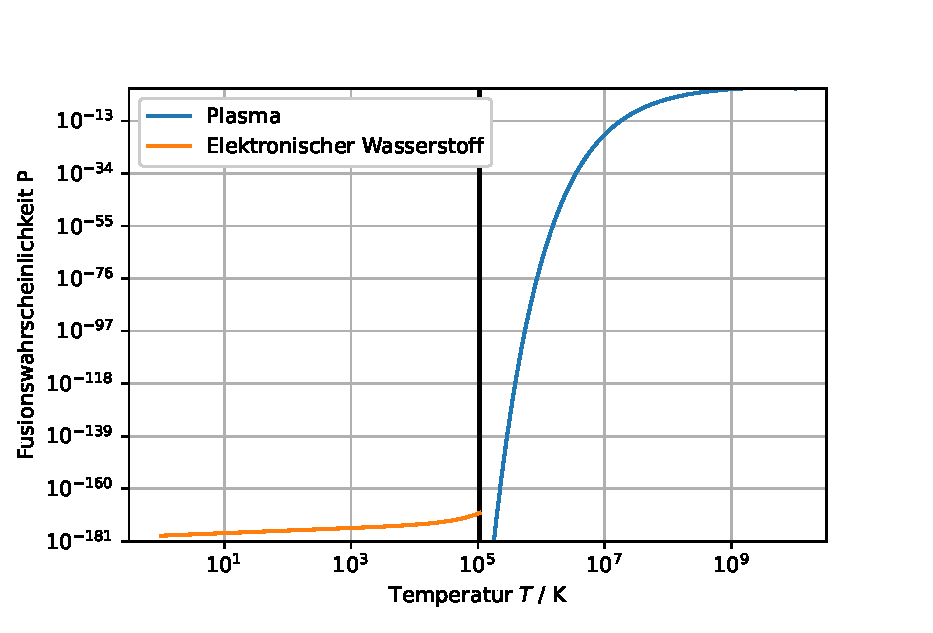
\includegraphics[width=0.8\textwidth]{images/Tunnelwahrscheinlichkeiten1.eps}
\end{frame}
